\documentclass[12pt]{beamer} %
\usepackage{amssymb,amsmath}
\usepackage[utf8x]{inputenc}
\usepackage{graphicx}
\setcounter{secnumdepth}{0}
\usetheme{Berkeley}
\usecolortheme{seagull}

\def\myEmail{hxr@hx42.org}
\def\InternalGithub{erasche}

\def\myGithub{@\InternalGithub}
\def\myGithubUrl{https://github.com/\InternalGithub}
\def\myName{Helena Rasche}

\logo{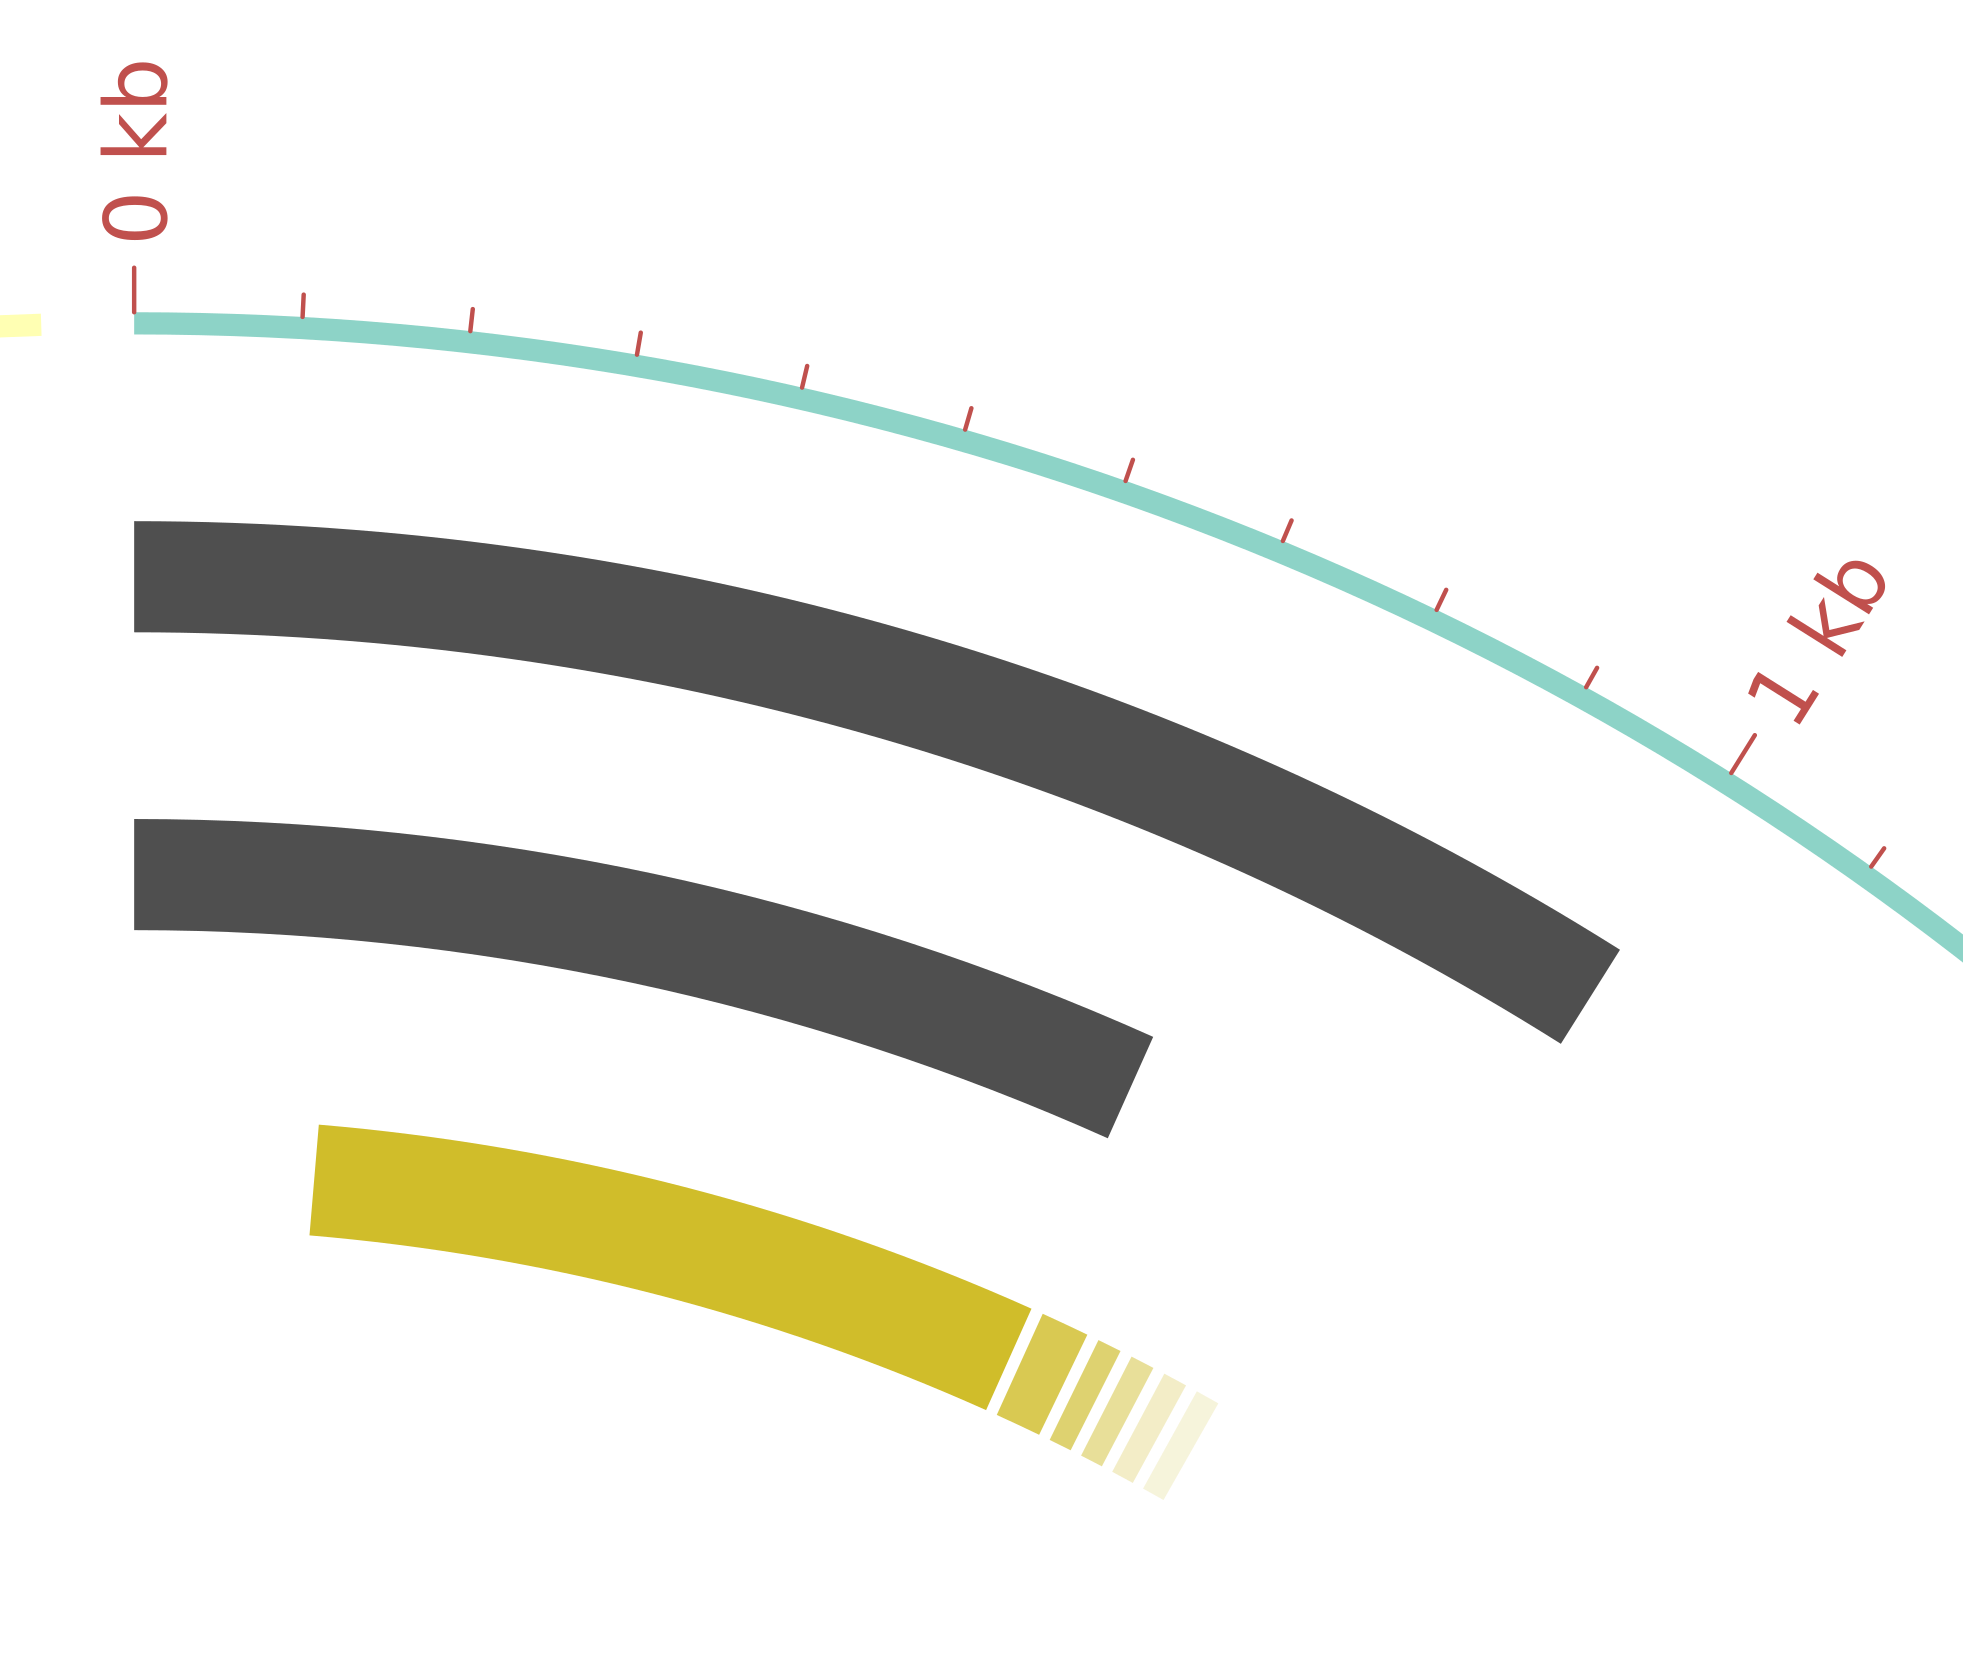
\includegraphics[width=1.5cm]{logo.png}}
\title[Circos]{A Generic Circos Galaxy Tool}
\author[\myName\\ \color{gray} \myGpgFingerprint]{\myName}
\date[\today]{\today}
\usepackage{hyperref}


\begin{document}
\frame{\titlepage}

\section{What is it?}
\begin{frame}{Circos is a Circular Data Plotter}
    \begin{itemize}
        \item Wide variety of standard plots (histograms, line graph, x-y plots, heatmaps,
            cytogenetic bands, ticks, grids, backgrounds, tiles, glyphs)
        \item Rule based plot customisation
        \item Chord Plots (ribbons, links)
    \end{itemize}
\end{frame}

{
  \usebackgroundtemplate{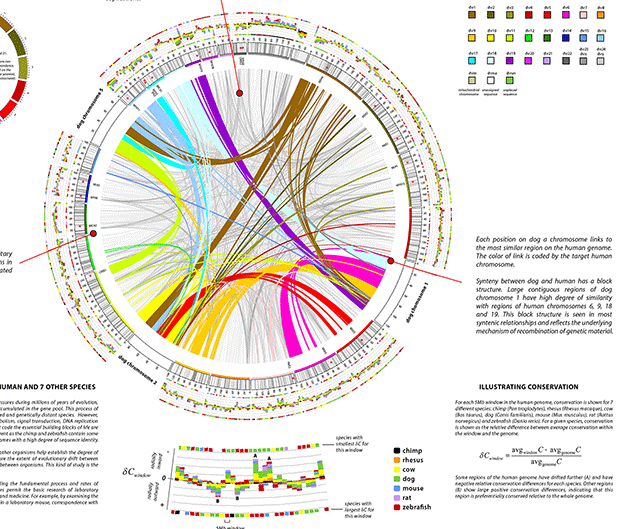
\includegraphics[height=\paperheight,width=\paperwidth]{circos.png}}
  \setbeamertemplate{navigation symbols}{}
  \begin{frame}[plain]
  \end{frame}
}

\section{Circos in Galaxy}
\begin{frame}{Why Circos as a Tool? Workflows!}
	\centering
	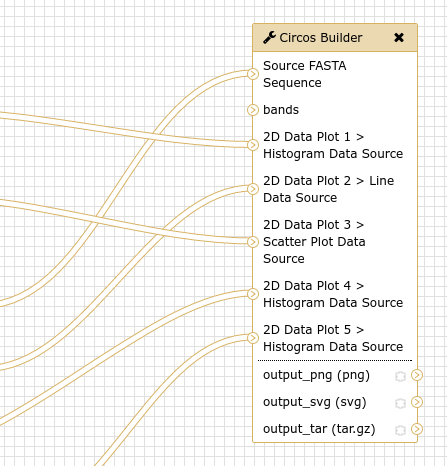
\includegraphics[width=\textwidth,height=\textheight,keepaspectratio]{2.png}
\end{frame}

\begin{frame}{In-depth Controls}
    \centering
    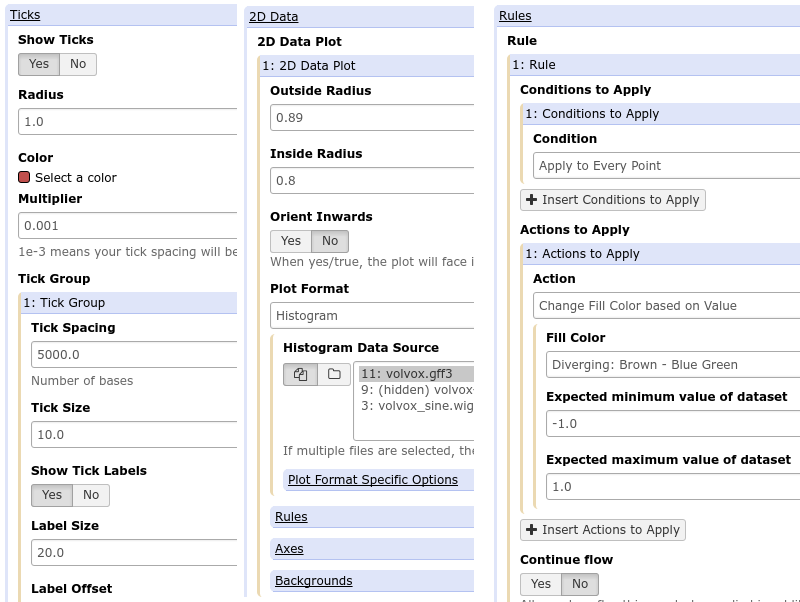
\includegraphics[width=\textwidth,height=\textheight,keepaspectratio]{3.png}
\end{frame}


\subsection{Screenshots}
{
  \usebackgroundtemplate{\includegraphics[height=\paperheight,width=\paperwidth]{1.png}}
  \setbeamertemplate{navigation symbols}{}
  \begin{frame}[plain]
  \end{frame}
}


\section{Roadmap}
\begin{frame}{Roadmap}
    \begin{description}
        \item[Completed:] Histograms, Line, Scatter, Heatmaps, Tiles, Axes, Backgrounds
        \item[In Progress:] Saskia Hiltemann has an open pull request adding support for Links and Ribbons
        \item[Future:] More advanced rule implementations, User facing documentation, Z-depth control, Move to \texttt{tools-iuc}
    \end{description}
\end{frame}


\section{Q\&A}
\begin{frame}{Q\&A}
    Thank you! \\\ \\
    \begin{center}
        \begin{tabular}{rl}
            \color{gray} Circos Tool Development      & \url{https://git.io/voN8N}\\
            \color{gray} GitHub           & \href{\myGithubUrl}{\myGithub}\\
            \color{gray} Twitter          & \href{\myTwitterUrl}{\myTwitter}\\
            \color{gray} Work Email       & \href{mailto:\myEmail}{\myEmail}%
        \end{tabular}
    \end{center}

    Bugs, Feature Requests welcome!
\end{frame}

\end{document}
